\label{sec:sysml:method}
Motivated by the success of social media user modeling using combinations of multiple posts by each user~\cite{andrews2019learning,noorshams2020ties}, we model posts on darknet forums using \textit{episodes}.
Each \textit{episode} consists of the textual content, time, and contextual information from multiple posts. 
A neural network architecture $f_{\theta}$ maps each episode to combined representation $e \in \mathbbm{R}^E$.
The model used to generate this representation is trained on various metric learning tasks characterized by a second set of parameters $g_{\phi}: \mathbbm{R}^E \xrightarrow[]{} \mathbbm{R}$.
We design the metric learning task to ensure that episodes having the same author have \textit{similar} embeddings.
Figure~\ref{fig:main_workflow} describes the architecture of this workflow and the following sections describe the individual components and corresponding tasks. 
Note that our base modeling framework is inspired by the social media user representations built by \citet{andrews2019learning} for a single task. 
We add meta-path embeddings and multitask objectives to enhance the capabilities of 
%this base model within 
\SYSMLmethodname{}. 
Our implementation is available at: \url{https://github.com/pranavmaneriker/SYSML}.

\begin{figure}[!htbp]
    \centering
    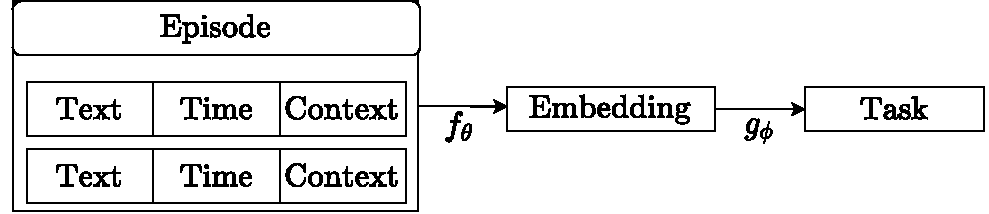
\includegraphics[width=\linewidth]{sysml/figures/MainFlowchart.pdf}
    \caption{Overall \SYSMLmethodname{} Workflow.}
    \label{fig:main_workflow}
\end{figure}

\subsection{Component Embeddings}
Each episode $e$ of length $L$ consists of multiple tuples of texts, times, and contexts 
\[
    e = \{(t_i, \tau_i, c_i) | 1 \leq i \leq L\} 
\]. 
Component embeddings map individual components to vector spaces. 
All embeddings are generated from the forum data only; no pretrained embeddings are used.

\noindent \textbf{Text Embedding} First, we tokenize every input text post using either a character-level or byte-level tokenizer. 
A one-hot encoding layer followed by an embedding matrix $E_t$ of dimensions $|V| \times d_t$ where $V$ is the token vocabulary and $d_t$ is the token embedding dimension embeds an input sequence of tokens $T_0$, $T_1$, $\dots, T_{n-1}$.
We get a sequence embedding of dimension $n \times d_t$. 
Following this, we use $f$ sliding window filters, with filters sized $F = \{2, 3, 4, 5\}$ to generate feature-maps which are then fed to a max-over-time pooling layer, leading to a $|F| \times f$ dimensional output (one per filter).
Finally, a fully connected layer generates the embedding for the text sequence, with output dimension $d_t$. 
A dropout layer prior to the final fully connected layer prevents overfitting, as shown in Figure~\ref{fig:kim_cnn}. 
\begin{figure}
    \centering
    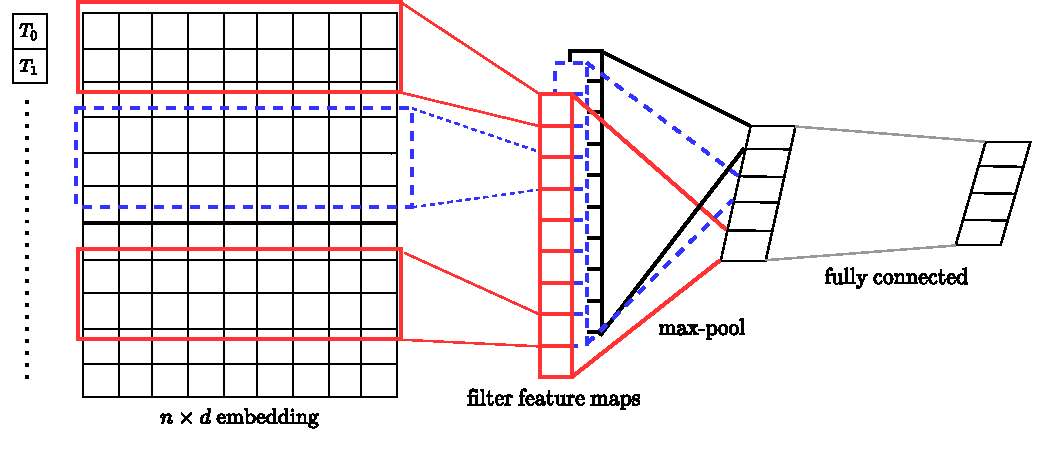
\includegraphics[width=\linewidth]{sysml/figures/TextCNN.pdf}
    \caption{Text Embedding CNN \cite{kim2014convolutional}.}
    \label{fig:kim_cnn}
\end{figure}

\noindent \textbf{Time Embedding} 
The time information for each post corresponds to when the post was created and is available at different granularities across darknet market forums. 
To have a consistent time embedding across different granularities, we only consider the least granular available date information (date) available on all markets.
We use the day of the week for each post to compute the time embedding 
by selecting the corresponding embedding vector of dimension $d_{\tau}$ from the matrix $E_w$.
%from a $7 \times d_{\tau}$ dimensional embedding matrix $E_w$ for a final embedding of dimension $d_{\tau}$.

\noindent \textbf{Structural Context Embedding} The context of a post refers to the threads that it may be associated with. 
Past work~\cite{andrews2019learning} used the subreddit as the context for a Reddit post.
In a similar fashion, we encode the subforum of a post as a one-hot vector and use it to generate a $d_c$ dimensional context embedding. 
In the previously mentioned work, this embedding is initialized randomly.
We deviate from this setup and use an alternative approach based on a \textit{heterogeneous graph} constructed from forum posts to initialize this embedding. 

\begin{definition}[Heterogeneous Graph]
A heterogeneous graph $G = (V, E, T)$ is one where each node $v$ and edge $e$ are associated with a `type' $T_i \in T$, where the association is given by mapping functions $\phi(v): V \rightarrow T_V$, $\psi(e): E \rightarrow T_E$, where $|T_V| + |T_E| > 2$
\end{definition}


The constraint on $T_{V,E}$ ensures that at least one of $T_V$ and $T_E$ have more than one element (making the graph heterogeneous). Specifically, we build a graph in which there are four types of nodes: user (U), subforum (S), thread (T), and post (P), and each edge indicates either a post of new thread (U-T), reply to existing post (U-P) or an inclusion (T-P, S-T) relationship.
To learn the node embeddings in such heterogeneous graphs, we leverage the metapath2vec~\cite{dong2017metapath2vec} framework with specific meta-path schemes designed for darknet forums. 
Each meta-path scheme can incorporate specific semantic relationships into node embeddings. 
For example, Figure~\ref{fig:metapath} shows an instance of a meta-path ‘UTSTU’, which connects two users posting on threads in the same subforum and goes through the relevant threads and subforum.
Our analysis is user focused; to capture user behavior, we consider \emph{all} metapaths starting from and ending at a user node. Thus, to fully capture the semantic relationships in the heterogeneous graph, we use seven meta-path schemes: UPTSTPU, UTSTPU, UPTSTU, UTSTU, UPTPU, UPTU, and UTPU. As a result, the learned embeddings will preserve the semantic relationships between each subforum, included posts as well as relevant users (authors). 
Metapath2vec generates embeddings by maximizing the probability of heterogeneous neighbourhoods, normalizing it across typed contexts.
The optimization objective is:
\begin{align*}
            \arg\max\limits_\theta \prod\limits_{v\in V} \prod\limits_{t\in T_v} \prod\limits_{c_t \in N_t(v)} p(c_t|v; \theta)
\end{align*}
Where $\theta$ is the learned embedding, $N_t(v)$ denotes $v$'s neighborhood with the $t^{th}$ type of node. 
In practice, this is equivalent to running a word2vec~\cite{mikolov2013efficient} style skip gram model over the random walks generated from the meta-path schemes when $p(c_t|v; \theta) = $ is defined as a softmax function. Further details of metapath2vec can be found in the paper by \citet{dong2017metapath2vec}.
\begin{figure}
    \centering
    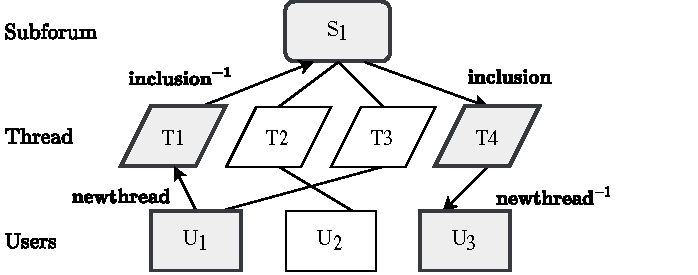
\includegraphics[width=\linewidth]{sysml/figures/metapathExample.pdf}
    \caption{An instance of meta-path ‘UTSTU’ in a subgraph of the forum graph.}
    \label{fig:metapath}
\end{figure}

\subsection{Episode Embedding}
The embeddings of each component of a post are concatenated into a $d_e = d_t + d_{\tau} + d_c$ dimensional embedding.
An episode with $L$ posts, therefore, has a $L \times d_e$ embeddings. 
We generate a final embedding for each episode, given the post embeddings using two different models.
In \textbf{Mean Pooling}, the episode embedding is the mean of $L$ post embeddings, resulting in a $d_e$ dimensional episode embedding.
For the \textbf{Transformer}, the episode embeddings are fed as the inputs to a transformer model~\cite{devlin2019bert,vaswani2017attention}, with each post embedding acting as one element in a sequence for a total sequence length $L$. 
We follow the architecture proposed by~\citet{andrews2019learning} and omit a detailed description of the transformer architecture for brevity (Figure~\ref{fig:emb_transformer} shows an overview).
Note that we do not use positional embeddings within this pooling architecture.
The parameters of the component-wise models and episode embedding models comprise the episode embedding $f_{\theta}: \left\{(t, \tau, c)\right\}^L \xrightarrow[]{} \mathbbm{R} ^ E$.

\begin{figure}
    \centering
    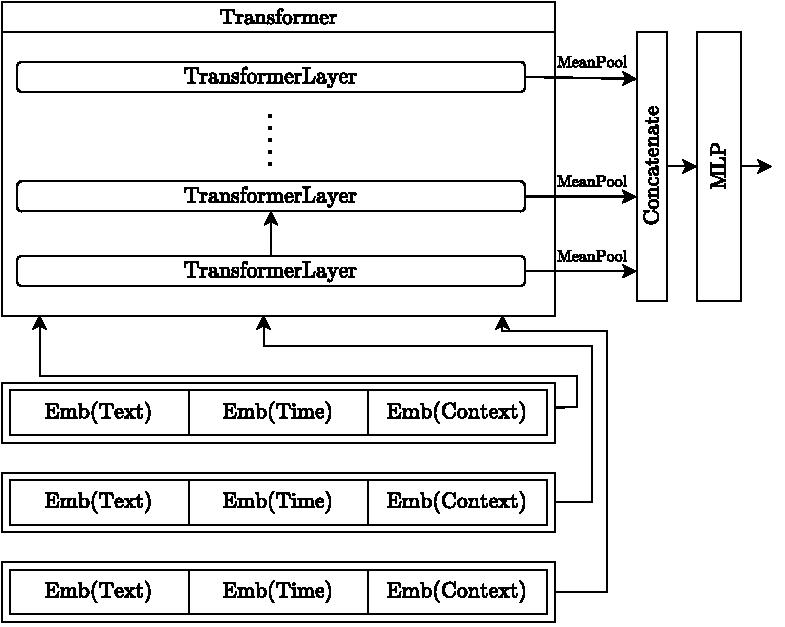
\includegraphics[width=0.7\linewidth]{sysml/figures/EmbeddingTransformer.pdf}
    \caption{Architecture for Transformer Pooling.
    %In mean pooling. The outputs from different layers are concatenated and then passed through an MLP to generate the final embedding for each episode.
    }
    \label{fig:emb_transformer}
\end{figure}

\subsection{Metric Learning}
\label{sec:framework:metric_learning}
An important element of our methodology is the ability to learn a distance function over user representations. We use the username as a label for the episode $e$ within the market $M$ and denote each username as a unique label $u \in U_M$.
Let $W =  |U_M| \times d_E $ represent a matrix denoting the weights corresponding to a specific metric learning method and let $x ^ * = \frac{x}{ || x||}$.
An example of a metric learning loss would be Softmax Margin, i.e., cross-entropy based softmax loss.
\begin{align*}
    P(u | e) = \frac{e^{W_{u} d_e}}{\sum\limits_{j=1}^{|U_M|}{e^{W_j d_e}}}
\end{align*}

We also explore alternative metric learning approaches such as Cosface (CF)~\cite{wang2018cosface}, ArcFace (AF)~\cite{deng2019arcface}, and MultiSimilarity (MS)~\cite{wang2019multi}. 

\subsection{Single-Task Learning}
The components discussed in the previous sections are combined together to generate  an embedding and the aforementioned tasks are used to train these models. 
Given an episode $e = \{(t_i, \tau_i, c_i) | 1 \leq i \leq L\}$, the componentwise embedding modules generate embedding for the text, time, and context, respectively.
The pooling module combines these embeddings into a single embedding $e \in \mathbbm{R}^E$. 
We define $f_\theta$ as the combination of the transformations that generate an embedding from an \textit{episode}.
Using a final metric learning loss corresponding to the task-specific $g_\phi$, we can train the parameters $\theta$ and $\phi$.
The framework, as defined in Figure~\ref{fig:main_workflow}, results in a model trainable for a single market $M_i$. 
Note that the first half of the framework (i.e., $f_\theta$) is sufficient to generate embeddings for episodes, making the module invariant to the choice of $g_\phi$. 
However, the embedding modules learned from these embeddings may not be compatible for comparisons across different markets, which motivates our multi-task setup. 

\subsection{Multi-Task Learning}

We use authorship attribution as the metric learning task for each market.
Further, a majority of the embedding modules are shared across the different markets.
Thus, in a multi-task setup, the model can share episode embedding weights (except context, which is market dependent) across markets. 
A shared BPE vocabulary allows weight sharing for text embedding on the different markets. 
However, the task-specific layers are not shared (different authors per dataset), and sharing $f_\theta$ does not guarantee alignment of embeddings across datasets (to reflect migrant authors). 
To remedy this, we construct a small, manually annotated set of labeled samples of authors known to have migrated from one market to another.
Additionally, we add pairs of authors known to be distinct across datasets.
The \textit{cross-dataset} consists of all episodes of authors that were manually annotated in this fashion.
The first step in the multi-task approach is to choose a market {($\mathcal{T}_M$)} or cross-market {($\mathcal{T}_{cr}$)} metric learning task $\mathcal{T}_i \sim \mathcal{T} =  \{\mathcal{T}_M, \mathcal{T}_{cr} \}$.
Following this, a batch of $N$ episodes $\mathcal{E} \sim \mathcal{T}_i$ is sampled from the corresponding task.
The embedding module generates the embedding for each episode $f_{\theta}^N: \mathcal{E} \xrightarrow[]{} \mathbbm{R}^{N \times E}$. 
Finally, the task-specific metric learning layer $g_{\phi}^{\mathcal{T}_i}$ is selected and a task-specific loss is backpropagated through the network. 
Note that in the \textit{cross-dataset}, new labels are defined based on whether different usernames correspond to the same author and episodes are sampled from the corresponding markets. 
Figure~\ref{fig:multitask_setup} demonstrates the shared layers and the use of \textit{cross-dataset} samples. 
The overall loss function is the sum of the losses across the markets: $\mathcal{L} = \underset{\mathcal{T}_i \sim \mathcal{T},\ \mathcal{E} \sim \mathcal{T}_i}{\mathbbm{E}}\left[\mathcal{L}_i(\mathcal{E})\right] $.
\begin{figure}
    \centering
    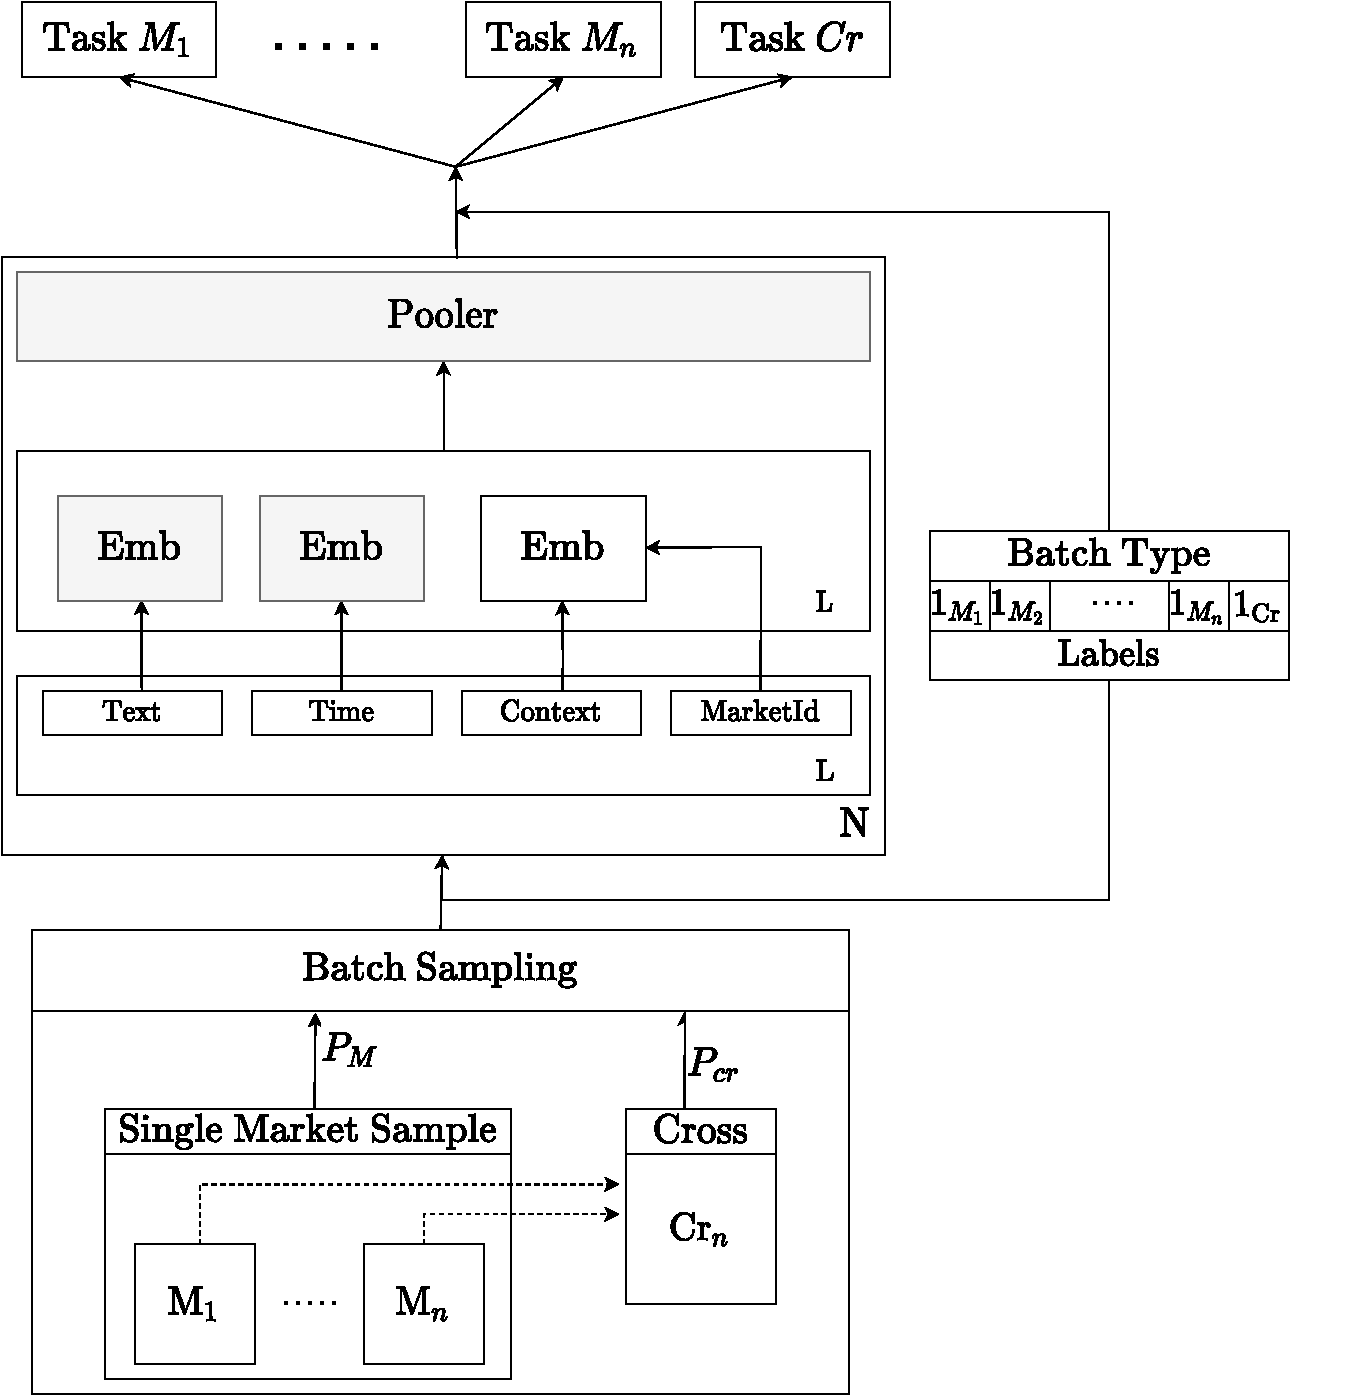
\includegraphics[width=0.8\linewidth]{sysml/figures/MultiTask.pdf}
    \caption{Multi-task setup. Shaded nodes are shared}
    \label{fig:multitask_setup}
\end{figure}
